 \begin{center}
 \textbf{
 %\dots
 \og 
La Sainte Trinité : Dieu en trois Personnes
 \fg
 %\dots
 }
 \end{center}

Le temps de Pâques prend fin avec la célébration de la Pentecôte qui est suivie par les célébrations de la Sainte Trinité, du Saint Sacrement et du Sacré Cœur de Jésus. Ces célébrations font ressortir la signification profonde des événements de Pâques. Dans la fête de la Sainte Trinité, nous célébrons le fait que Jésus n’est pas seul dans sa mission envers l’humanité. Il nous apporte un message du Père qui continue après son retour au Père. Et l’Esprit Saint poursuit cette mission avec le même message. Lui, non plus ne vient pas seul remplir sa mission, mais vient comme une aide envoyée à la fois par le Père et le Fils. C’est le mystère d’un seul Dieu qui se révèle en trois personnes : le Père, le Fils et le Saint Esprit. C’est de cette unité de Dieu que nous nous souvenons chaque fois que nous faisons le signe de la croix. La Sainte Trinité est le premier et le plus grand mystère de notre religion.
Ce mystère occupe une place prépondérante dans la vie de l’Église et des chrétiens. Car Dieu en se révélant, nous introduit dans l’intimité de son amour constant, invincible, inaltérable.

Toutefois, nous pouvons penser que le dogme de la Trinité peut paraître loin et ne pas toucher la vie. Au contraire celle-ci est la révélation du secret du vécu de la vie, de la sagesse sur la vie, sur la mort, sur l’amour, et elle nous dit : en tout premier, c’est un lien de liberté, c’est-à-dire une communion d’amour. Un seul Dieu en trois personnes : Dieu n’est pas en soi solitude, mais communion, l’océan de son essence vibre d’un infini mouvement d’amour, réciprocité, échange, rencontre, famille, fête.
Quand \og au commencement \fg{} Dieu dit: \og Faisons l’homme à notre image et ressemblance \fg{} l'image dont il parle n’est pas celle du Créateur, pas celle de l’Esprit, ni celle du Verbe éternel de Dieu, mais elle est toutes ces choses à la fois. La réalité d’amour qui est contenue dans ce premier et suprême Mystère de notre foi.
\begin{wrapfigure}{l}{1.3cm}
\vspace{-0.5cm}
	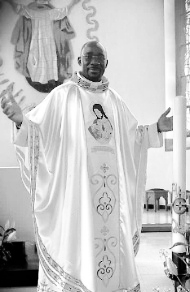
\includegraphics{../images/standing_daniel.png}
\end{wrapfigure}
Le Père, le Fils et le Saint Esprit sont Un, parce qu’ils sont amour et que l’amour est la force vivifiante absolue, que l’unité créée par l’amour est encore plus \og unité \fg{} qu’une unité purement physique. Le Père donne tout au Fils : le Fils reçoit tout du Père avec reconnaissance ; et le Saint Esprit est comme le fruit de cet amour réciproque entre le Père et le Fils.

\begin{flushright}
Bonne méditation !
\textit{Père  Daniel  ETTÉ}
\end{flushright}


